\documentclass[11pt,a4paper]{article}

% those are the packages loaded
\usepackage[T1]{fontenc}
\usepackage[utf8]{inputenc}
\usepackage{authblk}
\usepackage{hyperref}
\usepackage[xindy]{glossaries}
\usepackage{graphicx}
\usepackage{mathtools}
\usepackage{courier}
\usepackage[titletoc,toc,title]{appendix}
\usepackage{lineno}
\usepackage{tipa}
\usepackage{dirtytalk}
%\usepackage{fourier} 
\usepackage{array}
\usepackage{makecell}

\newcommand{\norm}[1]{\left\lVert#1\right\rVert}
\newcommand{\CC}{C\nolinebreak\hspace{-.05em}\raisebox{.4ex}{\tiny\bf +}\nolinebreak\hspace{-.10em}\raisebox{.4ex}{\tiny\bf +}}
\renewcommand\theadalign{cb}
\renewcommand\theadfont{\bfseries}
\renewcommand\theadgape{\Gape[4pt]}
\renewcommand\cellgape{\Gape[4pt]}
\renewcommand{\abstractname}{Executive Summary}

% this is for the title
\title{A neurocomputational model for spectro-temporal phonetic abstraction}

% those are the authors
\author[1]{Dario J. Dematties}
%\author[3]{Alejandro J. Wainselboim}
%\author[1,2]{B. Silvano Zanutto \thanks{Corresponding author \\ E-mail: silvano@fi.uba.ar}}

%those are the authors' affiliations
\affil[1]{Instituto de Ingeniería Biomédica, Facultad de Ingeniería, Universidad de Buenos Aires,
Ciudad Autonoma de Buenos Aires, Buenos Aires, Argentina}
%\affil[2]{Instituto de Biología y Medicina Experimental-CONICET,
%Ciudad Autonoma de Buenos Aires, Buenos Aires, Argentina}
%\affil[3]{Instituto de Ciencias Humanas, Sociales y Ambientales,
%Centro Científico Tecnológico-CONICET,
%Ciudad de Mendoza, Mendoza, Argentina}

% this command generates the glossary:
\makeglossaries

\loadglsentries{acronyms.tex}

% here is where the document starts
\begin{document}

\linenumbers

%\glsaddall

% the title is inserted here
\maketitle

%this is a kind of abstract called executive summary
\begin{abstract}
Basic linguistic units -such as vowels, consonants, syllables, etc-
are extracted and robustly classified by humans and other mammals
from complex acoustic streams in speech data.
Cortical structures -at different levels in the auditory pathway as well as at higher levels-
respond selectively to phonetic features embeded in acoustic stimuli.
In this research proposal we introduce a neurocomputational,
completely unsupervised and biologically plausible model
which establishes a new approach for deep feature extraction
architectures in order to assist supervised phonetic classification
techniques.
The model we present here is entirely parallelized and scalable.
In coordination with \gls{hpc} assistance from Argonne National Laboratory
we will execute experimental tests in \gls{hpc} facilities at Argonne.
In this context, I will attend \gls{mpi} Tutorials to be held at
the Argonne \gls{tcs} Center, whose tutors belong to the group
that invented and currently maintain \gls{mpi}.
Beyond the benefits provided to my project,
this experience will also favor my future application as a candidate
for the next \gls{atpesc} edition. 
We also plan to work with Assistant Computer Scientist at Argonne
in data analysis and visualization to explore visualization techniques
in order to inspect closely and thoroughly the evolution of
training and testing stages
in our systems.
This project will receive mentoring from the Department of Neurobiology at
University of Chicago from which we will receive state-of-the-art
techniques in order to create complete and comprehensive maps of the brain.
Our research will also receive mentoring in language processing
from Departmental of Computing at
Loyola University Chicago.
The objective of our research is to develop novel deep phonetic
feature extraction techniques based on relevant neurophysiological
cortical mechanisms.
With the implementation of these new approaches, we expect to
achieve phonetic classification performances at the level of state-of-the-art deep learning architectures. 
With these results, we aim to draw attention 
towards neurophysiological characteristics which are
relevant for information processing in perception.
\end{abstract}



















% this is the first section in my paper; it is called "Introduction"
\section{Introduction}

It is well known that human beings have the ability to reliably discriminate phonemes
as well as other linguistic units by categorizing them,
in spite of considerable variability across different speakers
with different pitches and prosody, even in noisy and reverberant
environments.
On the other hand, it has also been shown that trained animals
are able to discriminate phoneme
pairs categorically and to generalize in novel situations
\cite{kuhl_1975, kuhl_1983, kluender_1998, pons_2006, hienz_1996, dent_1997, lotto_1997}. \\

To understand how phonetic categories and word-like units
are acquired, several computational theories have been developed.
In the context of such theories, the main idea has
been to explain relevant aspects of phonetic acquisition neglecting details
about how the brain might provide such
computations \cite{rasanen_2012}. \\

Lack of invariance phenomenon in speech perception
\cite{appelbaum_1996}
seems to be one of those scientific problems which
cannot be solved by spontaneous human reasoning,
given the immense amount of interrelated variables
involved in phonetic categorization processes. \\

In that sense, deep learning architectures have shown
unprecedented performance in the assistance of
conventional machine learning techniques, which for decades 
required careful engineering
in order to reach an effective feature extraction design
\cite{lecun_2015}. \\

Nevertheless, artificial neural networks do not take into account
remarkable biological aspects discovered during the last years
in the area of neuroscience.
Certain biological principles could be crucial in terms of
information processing in the brain and they could
provide us with matchless strategies in order to extract
relevant information from a raw set of stimuli
during perception. \\

The approach in this research is to gather
potentially relevant biological aspects which could be
significant in terms of information processing
in the mammalian auditory cortex. We intend to test those principles
with computational models which could
perform in similar levels to state-of-the-art pattern classification techniques. \\

This work does not aim to replicate 
neuro-physiological mechanisms with precision nor to get a detailed reproduction
of human cortical tissue; that is beyond the scope of our research. 
In contrast, it aims to parsimoniously incorporate cortical
neurophysiological mechanisms letting the models
speak by themselves.
The biological mechanisms, whose feature extraction
properties show significant performance
in invariant phonetic classification tasks, will be
highlighted for a future observation in upcoming researches. \\

In other words, this work seeks for novel computational solutions
to automate feature extraction processes as a means
of assistance in spectro-temporal phonetic classification. \\




















\section{Working Plan During the Permanence at Argonne}

We have implemented a neurocomputational model whose biological plausibility
allows us to test neurophysiological hypotheses incorporated in the algorithms.
With the desired number of layers, our model abstracts phonological features
in a completely unsupervised fashion.
The input is composed by a series of words which are processed by another algorithm
in order to feed the model.
The phonetic features extracted by the model have the function of improving
the performance of supervised pattern classification techniques
whose main objective is to test the level of invariance achieved by the model's layers. \\

The objectives pursued in the present work lead to two main challenges.
First, the correct identification and pertinent selection of those neurophysiological
mechanisms in the auditory pathway, and the way in which they must be incorporated
in the algorithms.
Regarding this issue, during the permanence at Argonne National Laboratory (https://www.anl.gov/),
this project will count on the
research mentoring by Narayanan Kasthuri's lab
from the Department of Neurobiology at University of Chicago.
This group is currently facing one of the biggest challenges in the world by 
creating a complete and comprehensive map of the mammalian brain.
On the other hand, this project will also count on the mentoring by
George K. Thiruvathukal from the Department of Computer Science at
Loyola University Chicago,
in order to achieve a correct algorithmic formulation and implementation.
Professor Thiruvathukal's specialty area includes
parallel and distributed systems, software engineering, programming languages and operating systems.
Dr. Thiruvathukal's early research involved object-oriented approaches to parallel programming
and the development of object models with parallel programming, mostly based on C and \CC  on Unix platforms. \\

Second, the
unsupervised training and testing phases for model instances from moderate to small sizes
could take between 12 and 24 hours.
Input computation can take up to 1 hour.
Memory is a critical factor in such computation,
even for very small corpora of 500 words.
Likewise, the supervised training phase for \gls{libsvm} can take 2 or more hours.
Memory and computational capability shortages obstruct our possibilities of producing
the amount of tests necessary over different model configurations in order to find correct
parameter combinations.
The size of the model instances as well as the experiments we can execute
are remarkably limited by our computational resources.
During the stay at Argonne we will have access
to high performance computing capabilities of unrivalled level in the world.
Among them, we will have access to supercomputers
ranked at the 9th (Mira) and 16th (Theta) positions in the Top500
(https://www.top500.org/list/2017/06/?page=1).
In this context, we will also count on the mentoring advice from Silvio Rizzi
who is an Assistant Computer Scientist at the Argonne Leadership Computing Facility.
Dr. Rizzi will assist our project with \gls{hpc} technical support.
Hence, we will be able to test model configurations
with dimensionalities and sizes which we have no access to in our current context.
Emergent properties could arise from the enormous amount of parameter combinations in the design
of those new instances.
Surrounded by this framework, we plan to execute an ensemble of jobs,
supervised by a genetic algorithm in which we will run several model instances
in order to automate the process of parameter selection guided by the
classification performance of the instances. \\

In addition to the orders of magnitude in the number of advantages and variants for 
model parametrization and scalability, we have to consider new experimental
possibilities offered by such working conditions.
After getting the correct combination of parameters for the model configurations,
we will be able to test the model performance in standardized corpora such us
\gls{timit} (https://catalog.ldc.upenn.edu/ldc93s1), whose experimental tests
are not feasible with our resources. \\

Given the temporal requirements, we are probably in the best conditions to gain
considerable benefits from the time we would spend at Argonne.
We count on a model implementation that is completely parallelized. %TODO Ale think it must be "count with"
The parallelization in OpenMP \gls{api} does not affect the original sequential implementation
of the code. This parallelization approach allows automatic scalability and a completely serialized
compilation if necessary. \\

Such applications will return feature vectors with orders of magnitude larger than those obtained with our current tests.
In this respect, we plan to pursue extensions to the \gls{libsvm} soft -as \gls{liblinear}- which can be implemented in
shared-memory systems to reduce the training time dramatically. \\

The software used to manipulate all the data processed and produced by the model
is implemented under \gls{gnu_octave} (https://www.gnu.org/software/octave/).
In cases of vector with high dimensionality -as we mentioned above-
we will have to parallelize such code.
\gls{gnu_octave} offers packages which enable parallelization in shared memory systems. \\

The significance of visual observation in scientific data becomes apparent
when we enumerate the overwhelming amount of examples in this respect.
Besides all the evidence in favour of this policy, we will cite
a compelling example from fractional calculus notation \cite{Miller_1993}.
From this example it should be clear that, as visual animals,
visual observation brings us unparalleled advantages. \\

\say{The choice of a precise notation for the fractional calculus cannot
be minimized. For as we shall see, some of the power and elegance of
the fractional calculus rests in its simplified notation. The abridged
manner of representing these defining integrals may seem to be a
trivial matter; but the advantage of a simple notation has been the
source of many profound discoveries not obvious by other means.} \\

\begin{figure}[h!]
  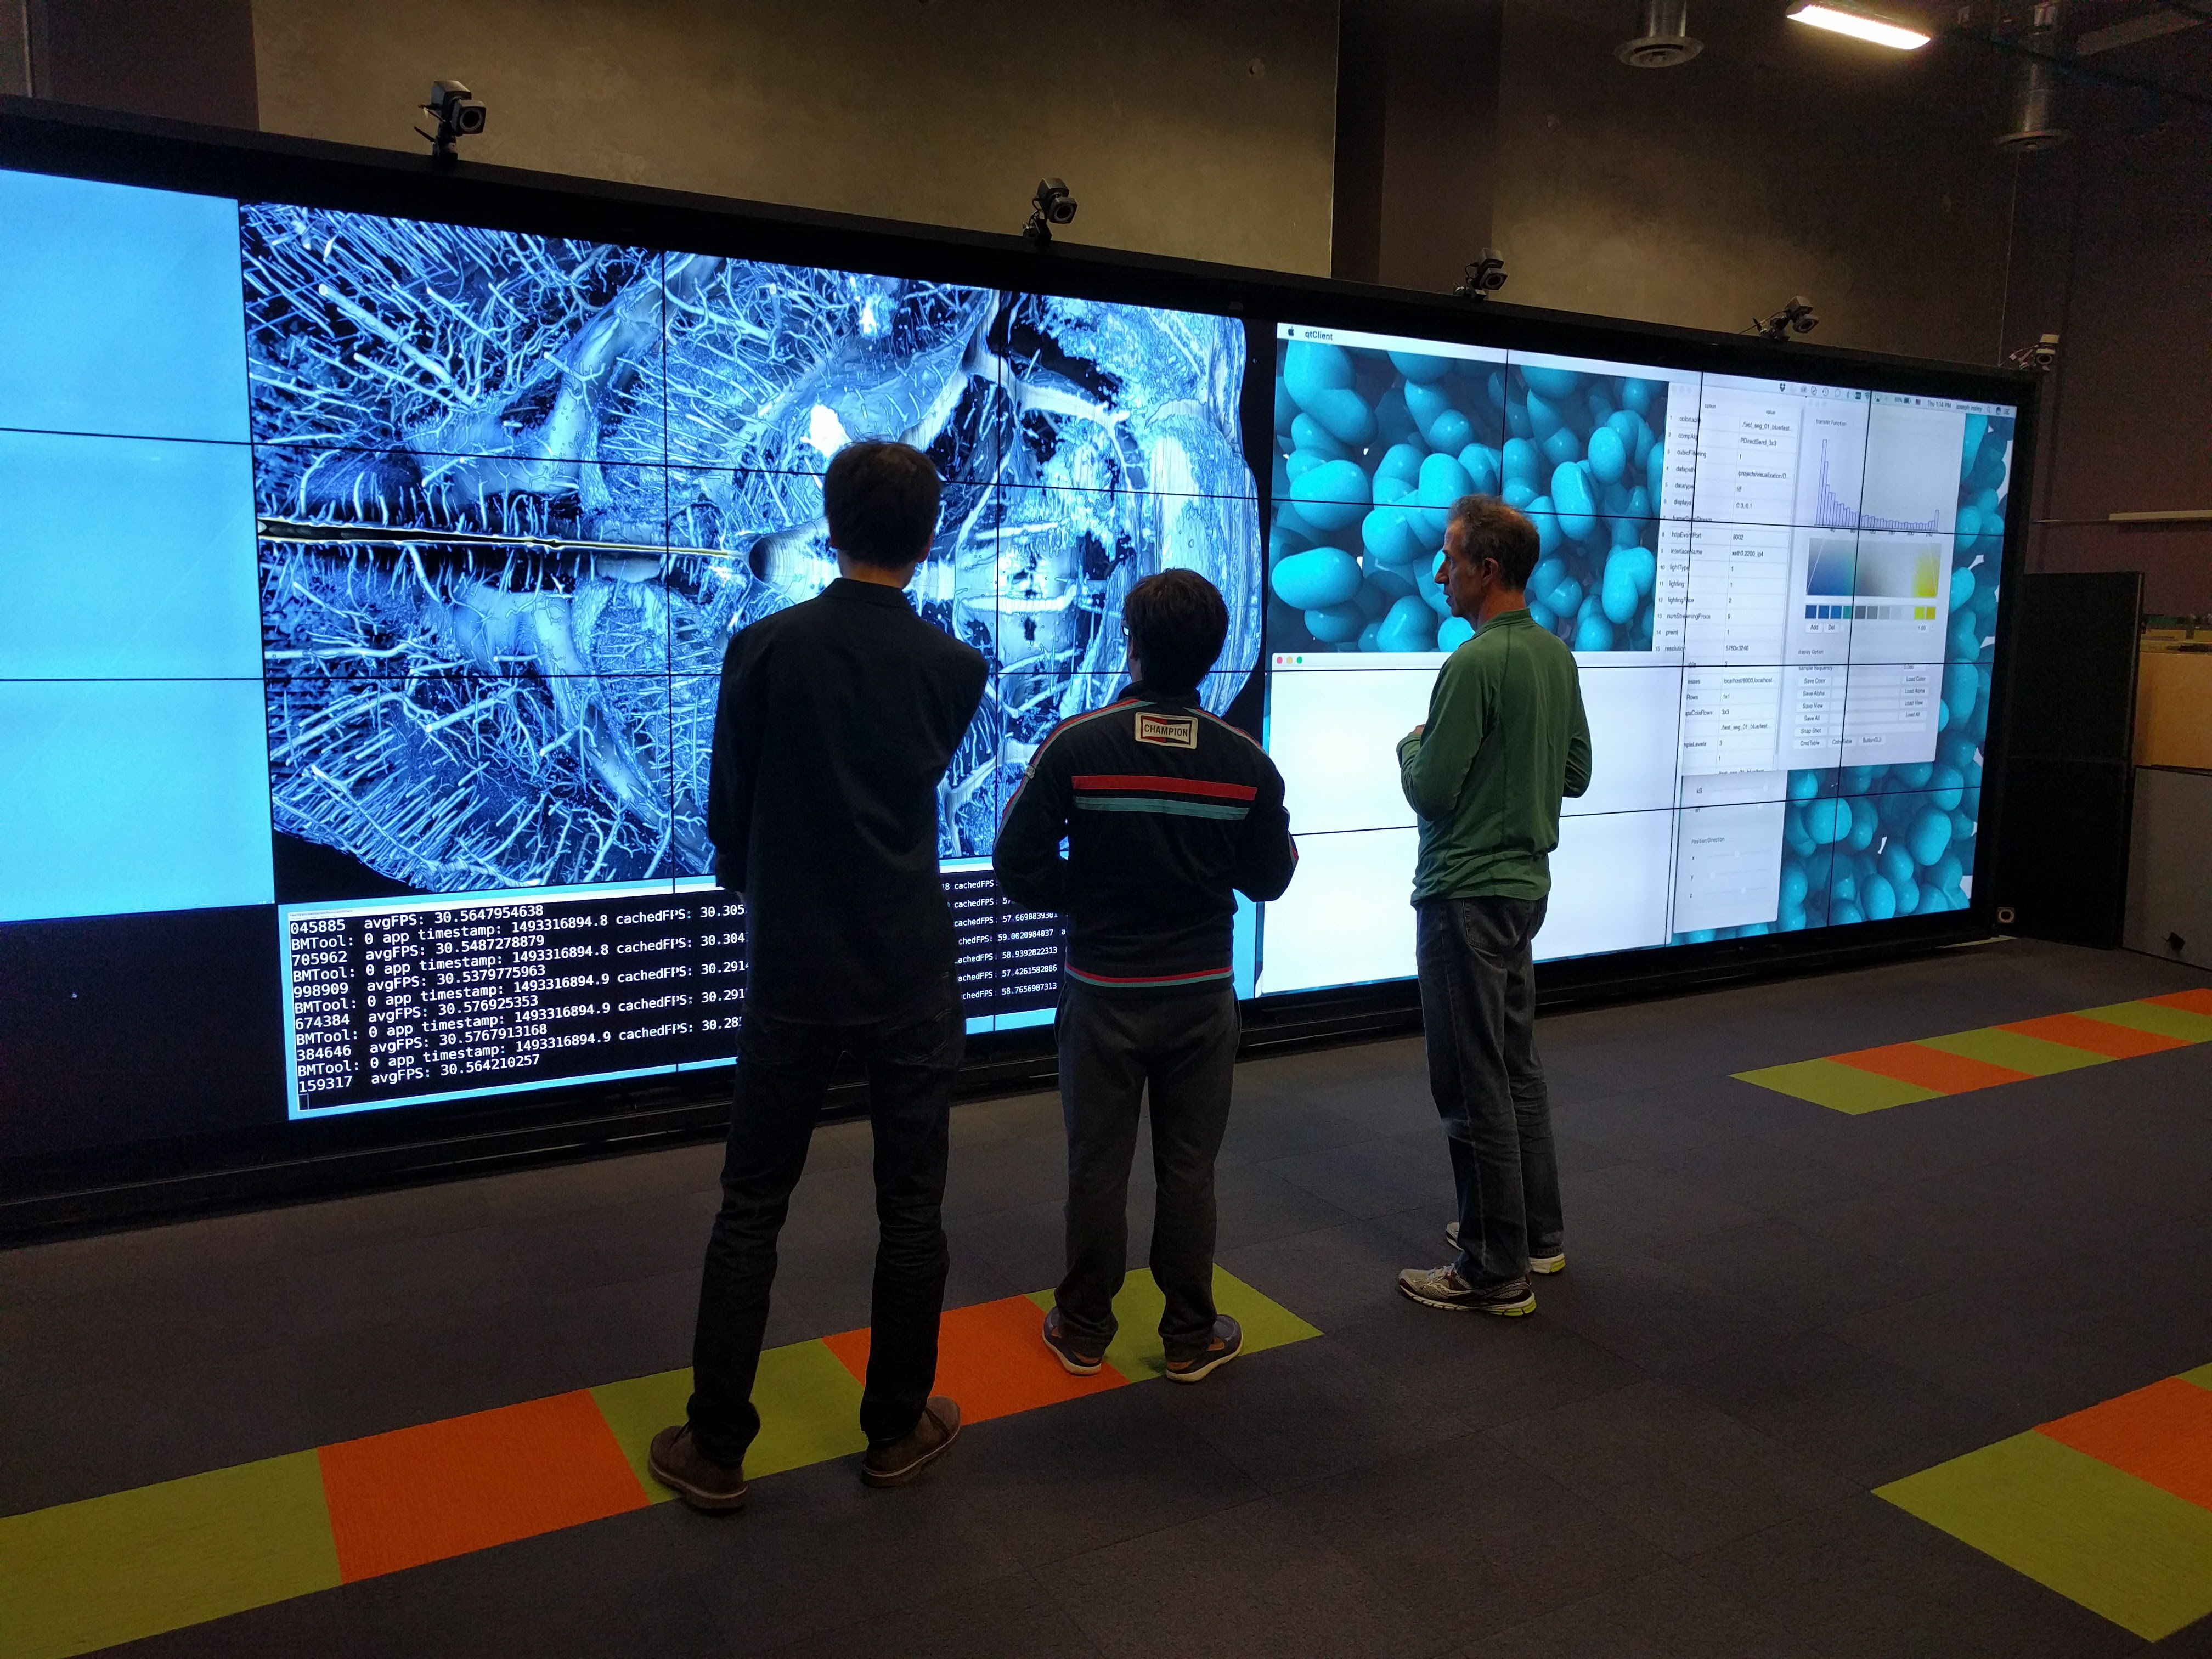
\includegraphics[width=\linewidth]{visualization.jpg}
  \caption{Large-Scale Computing and Visualization on the Connectomes of the Brain. %
  Image courtesy Joe Insley, Silvio Rizzi, Argonne Leadership Computing Facility}
  \label{connectome}
\end{figure}

The way in which we visually represent our data is crucial for the success of
our project.
Regarding this aspect, we will be assisted by Argonne Assistant Computer Scientists
in order to get the best options for the visual representation of our data.
We plan to visualize the training and processing evolution of hundreds of thousands
of units with millions of connections through the use of large tiled displays.
Figure \ref{connectome} shows a large-scale visualization of the connectomes.
The image technique is based on X-Ray extended tomography (or Mosaic Tomography)
with 1 micron resolution performed at the beamline 32-ID-C on the Advanced Photon Source.
The segmentation is tensor flow based in order to 
extract features like cell bodies, myelinated axons and blood vessels.
The image resolution is obtained through multiple images acquired
and stitched together. Image on Figure \ref{connectome} comes from
downsampled segmented dataset at 2Kx1Kx2K.
Full resolution is about 20Kx20K pixels per slice. 
In Table \ref{tentative-plan} we have drawn a tentative working plan to be carried on
at Argonne. \\

We aim to publish this work outcomes in international high impact factor journals 
similar to Plos One or Plos Computational Biology. \\

% this is a table with a tentative working plan at Argonne
\begin{table}[]
\centering
\caption{Tentative working plan}
\label{tentative-plan}
\resizebox{\textwidth}{!}{\begin{tabular}{|l|l|l|}
\hline
\multicolumn{3}{|l|}{\textbf{Week 1}} \\ \hline
\textbf{Milestone} & \textbf{Details} & \textbf{Date and Status} \\ \hline
\thead{Setup} & \thead{Set up my personal accomodation and workspace.} & -- \\ \hline
\thead{Site access} & \thead{Argonne National Laboratory is a controlled access facility, and approval for site access is required. \\ All visitors must be pre-authorized before being allowed on the Argonne site.} & -- \\ \hline
\thead{Safety Training} & \thead{Before performing work at Argonne, I must take certain orientation and safety training courses.} & -- \\ \hline
\multicolumn{3}{|l|}{\textbf{Week 2}} \\ \hline
\thead{Meeting} & \thead{First meeting with \gls{hpc} stuff. Initial work coordination.} &  \\ \hline
\thead{Initial tests} & \thead{Test of initial model configurations with serial supervised classification algorithms.} &  \\ \hline
\thead{Parallelization} & \thead{Parallelization of Octave code for supervised algorithm classification assistance. Use of package Parallel for Octave. \\ The classification code is for a reduced number of dimensions and examples. Use of \gls{libsvm}.} &  \\ \hline
\thead{Session of Tests} & \thead{Session of tests with a greater amount of examples and vector features} &  \\ \hline
\multicolumn{3}{|l|}{\textbf{Week 3}} \\ \hline
\thead{Meeting} & \thead{Meeting at Department of Neurobiology.} &  \\ \hline
\thead{Meeting} & \thead{Meeting at Department of Computer Science.} &  \\ \hline
\thead{\gls{liblinear} implementation} & \thead{Multi-core \gls{liblinear} initial implementation.} &  \\ \hline
\thead{Conference} & \thead{Conference of model neurophysiological and computational aspects.} &  \\ \hline
\thead{Meeting} & \thead{Post-Conference Meeting at Department of Computer Science.} &  \\ \hline
\multicolumn{3}{|l|}{\textbf{Week 4}} \\ \hline
\thead{Meeting} & \thead{Post-Conference Meeting at Department of Neurobiology.} &  \\ \hline
\thead{\gls{mpi} Tutorial} & \thead{\gls{mpi} Tutorial Initialization} &  \\ \hline
\thead{Session of Tests} & \thead{Preparation of session of tests with \gls{liblinear}. \\ Massive amount of examples and vector featues.} &  \\ \hline
\thead{\gls{mpi} Tutorial} & \thead{\gls{mpi} Tutorial course.} &  \\ \hline
\multicolumn{3}{|l|}{\textbf{Week 5}} \\ \hline
\thead{Session of Tests} & \thead{Tests with \gls{liblinear}. Massive amount of examples and vector featues.} &  \\ \hline
\thead{\gls{mpi} Tutorial} & \thead{\gls{mpi} Tutorial course.} &  \\ \hline
\thead{Session of Tests} & \thead{Tests with ensemble of jobs in order to make a parameters' sheep} &  \\ \hline
\thead{\gls{mpi} Tutorial} & \thead{\gls{mpi} Tutorial course.} &  \\ \hline
\multicolumn{3}{|l|}{\textbf{Week 6}} \\ \hline
\thead{Session of Tests} & \thead{Tests with ensemble of jobs together with genetic algorithms in order to extract best parameter configurations.} &  \\ \hline
\thead{\gls{mpi} Tutorial} & \thead{\gls{mpi} Tutorial course} &  \\ \hline
\thead{Session of Tests} & \thead{Tests with ensemble of jobs together with genetic algorithms \\ in order to extract best parameter configurations. \\ Tests performed on \gls{timit} database.} &  \\ \hline
\thead{\gls{mpi} Tutorial} & \thead{\gls{mpi} Tutorial course.} &  \\ \hline
\multicolumn{3}{|l|}{\textbf{Week 7}} \\ \hline
\thead{Meeting} & \thead{Meeting at Department of Neurobiology in order to discuss results and eventual modifications.} &  \\ \hline
\thead{\gls{hpc} Meeting} & \thead{Meeting at \gls{hpc} laboratory in order to start the migration of the central code to \gls{mpi}. \\ Preliminary analysis of visualization issues.} &  \\ \hline
\thead{\gls{mpi} Migration} & \thead{Start the migration of the model central code to \gls{mpi} \gls{api}.} &  \\ \hline
\thead{Meeting} & \thead{Meeting at Department of Computer Science in order to discuss results, eventual modifications and \gls{mpi} migration.} &  \\ \hline
\thead{MPI Migration} & \thead{Migration of the model central code to \gls{mpi}.} &  \\ \hline
\thead{Session of Tests} & \thead{First tests of the code in \gls{mpi}.} &  \\ \hline
\multicolumn{3}{|l|}{\textbf{Week 8}} \\ \hline
\thead{Visualization Issues} & \thead{Start implementation of model evolution visualization.} &  \\ \hline
\thead{Octave \gls{mpi}} & \thead{Initial migration of Octave code through the use of \gls{mpi} for Octave.} &  \\ \hline
\thead{Meeting} & \thead{Meeting at Department of Computer Science in order to discuss results, eventual modifications and Octave \gls{mpi} migration.} &  \\ \hline
\thead{Session of Tests} & \thead{Running tests of complete model implementation in \gls{mpi} on \gls{timit} database} &  \\ \hline
\thead{Results Assemblage} & \thead{Assemblage of results. Data analysis. Data presentation.} &  \\ \hline
\multicolumn{3}{|l|}{\textbf{Week 9}} \\ \hline
\thead{Meeting} & \thead{\gls{hpc} meeting. Visualization issues. Final adjustments.} &  \\ \hline
\thead{Tests Sessions} & \thead{Tests of the visualization. Results compilation.} &  \\ \hline
\multicolumn{3}{|l|}{\textbf{Week 10}} \\ \hline
\thead{Meeting} & \thead{Meeting at Neurobiology and \gls{hpc} departments in order to discuss data visualization.} &  \\ \hline
\thead{Meeting} & \thead{Meeting at Department of Computer Science.} &  \\ \hline
\thead{Results Assemblage} & \thead{Visualization. Results assemblage.} &  \\ \hline
\multicolumn{3}{|l|}{\textbf{Week 11}} \\ \hline
\thead{Final Conference} & \thead{Conference with the complete data compilation.} &  \\ \hline
\thead{Meeting} & \thead{Meeting at \gls{hpc}, Computer Science and Neurobiology's laboratories \\ in order to give initial layout to tentative publication.} &  \\ \hline
\thead{Publication} & \thead{Start publication preparation.} &  \\ \hline
\multicolumn{3}{|l|}{\textbf{Week 12}} \\ \hline
\thead{Wrap up} &  &  \\ \hline
\thead{Wrap up} &  &  \\ \hline
\thead{Wrap up} &  &  \\ \hline
\end{tabular}}
\end{table}














\section{Expected Outcomes and Benefits}

We are convinced that, in order to get truly general 
artificial intelligent agents, we need to reverse-engineer
-at least- those physiological brain mechanisms of relevance
for information processing in perception.
The objectives sought in the proposed research
determines unexplored challenges in the automatic deep
feature extraction field.
We seek for unprecedented techniques to get
phonetic classification performance improvements
through the use of neurophysiological data that has
not been used in current deep learning technologies. \\

Invariance is the holy grail of pattern classification,
and tiny improvements -even in some small fractions
of percentage- are highly appreciated in this area.
We are seeking a completely new approach in the world of
artificial phonetic perception but, apart from that,
the contributions that we could obtain from our
experimental results could establish new directions
in terms of the relevance attributed
to certain physiological
structures for information processing in the brain.
Furthermore, the relevance of our future discoveries
could cross the frontiers of auditory perception
and influence other modalities
such as visual and somatosensory ones. \\

Having the possibility of working with professor
Kasthuri from the Department of Neurobiology,
professor Thiruvathukal from the  Loyola University of Chicago and
Dr. Silvio Rizzi from Argonne National Laboratory and University of Chicago,
and given the favorable relationships available through the
INTERNATIONAL RESEARCH COOPERATION BETWEEN THE MINISTRY OF SCIENCE,
TECHNOLOGY AND PRODUCTIVE INNOVATION
OF THE ARGENTINE REPUBLIC
AND
THE UNIVERSITY OF CHICAGO,
represents unparalleled prospects for the
evolution of this work, my professional career
and long lasting scientific cooperation
relationships in the future. \\

























\section{Previous Research}

Among the computational theories developed to understand
human phonetic acquisition, some models bypass the initial
speech signal processing and,
instead of dealing with the complexity and variability of real speech
at the prelexical level, they use an artificial, often hand-crafted, 
idealized discrete (prelexical) representation of the acoustic
signal as an input to the lexical level \cite{scharenborg_2010}.
In other works \cite{dominey_2000}, although some biological observations are made,
the input components are syllable representations from specific corpora.\\

In the works by de Boer and Kuhl \cite{boer_2003} and Vallabha, McLelland, Pons,
Werker and Amano \cite{vallabha_2007}, the models classify some vowels
through statistical mechanisms which take into account formant components
and \gls{vl}.
In Toscano and McMurray \cite{toscano_2010},
statistical methods are used to classify consonantal phonetic
characteristics, by means of \gls{vot},
\gls{vl}, pitch and first formant onset frequency. \\

The statistical methods used in these works make
different features extracted from acoustic speech signals
interrelate.
Those features are carefully weighted
through human engineering and domain expertise
which evaluate their relevance in order to include them
in the computations.
Some features, as \gls{vl} and \gls{vot},
refer to highly abstract dynamic characteristics
which are taken
as available parameters without any previous natural
processing.\\

We consider the possibility of the existence of other
features which can escape human expertise.
Furthermore, some hidden features could be a constituent
part of those abstract features evaluated by humans. \\

In this respect, deep learning approaches have gained significant interest as a
way of building hierarchical representations from unlabeled data.
Convolutional deep belief networks have been applied to audio data and,
such architectures have been empirically evaluated on various audio classification
tasks. In the case of speech data, it was shown that the learned features corresponded
to phones/phonemes \cite{Lee:2009:UFL:2984093.2984217}. \\

In Kouki et al. \cite{kouki_2010},
the use of \gls{mfcc}
strategy presupposes a more biologically accurate input stream,
though the cepstrality in such coefficients does not reflect
-under our point of view-
the responsive air cells in front of cochlear vibration.
In a subsequent work, Kouki et al. \cite{kouki_2011},
designed a method to separate “stable” and “dynamic” speech
patterns. \\

All the above-cited works lack biological plausibility.
Regarding this point, in the last few years a compelling
theoretical framework has been developed.
In this theory, certain hypotheses about the role of
the neocortex in the mammalian brain are given in an
approach called \gls{mpf}
\cite{hawkins_2004}.
This approach is based on evidence
which supports the idea that there are fundamental
mechanisms which underly a common neocortical
structure and its connectivity.
In a recent work, it was shown that a neuron with
several thousand synapses could recognize hundreds
of independent patterns of cellular activity even
in the presence of large amounts of
noise and pattern variation.
A neuron model was proposed in which by means of
the combination of proximal and distal dendrites
it could predict its activation in hundreds of independent contexts.
Through simulation procedures, it was shown that a network
scaled well and operated robustly over a wide range of parameters as long as it
used a sparse distributed code of cellular activations.
It was concluded that pyramidal neurons with thousands of
synapses, active dendrites, and multiple integration zones
created a robust and powerful
sequence memory \cite{hawkins_2016}. \\

We favour an approach similar to the one taken in \cite{hawkins_2016}.
We support the idea that in order to design truly powerful machine
learning techniques,
it is necessary to gather those biological characteristics which are
relevant -regarding information processing- to highly
robust invariant pattern representation capabilities. \\













\section{Theoretical Framework and Hypotheses to be Tested}

Cortical cells are aligned into restricted domains for common receptive field locations,
which represent different sensory modalities and are composed by neural cells of identical
salient physiological characteristics.
V. Mountcastle proposed such structures as elementary units for structural organization
in the somatic cortex and called them cortical columns \cite{mountcastle_1955, mountcastle_1957}.
The first confirmatory experimental results for this phenomenon came from Hubel and Wiesel’s
discoveries \cite{hubel_1962, hubel_1968}.
Margins in column diameter are between 300 and 600 $\mu m$; even
among different species whose brains differ in volume by a factor of $10^3$.
The evolutionary cortical brain expansion is achieved through the expansion in
cortical surface area by means of an increase in the number of cortical columns
and not by the increase in individual column size \cite{rakic_1995}.
These facts suggest that cortical tissue is organized in a modular and uniform structure.
In accordance, Mountcastle suggested in 1978 that there could be
a unique cortical algorithm replicated throughout the neocortex
\cite{mountcastle_1978}.\\

Linden and Schreiner proposed that although auditory
cortical circuits have some unique characteristics,
their similarities with other sensory regions -such as visual or somatosensory cortex-
seem to be much more categorical \cite{linden_2003}.
They proposed a series of analogies:
first, at the sensory level, the cochlear one-dimensional frequency map
could be analogue to the two-dimensional spatial maps which are found
in the retina or body surface.
Second, the tonotopic maps found in the auditory system could be analogue to the
retinotopic and somatotopic organization found in visual and somatosensory cortices,
respectively.
Frequency tuning curves in the auditory system could correspond to inhibition of
spatial surrounding boundaries in visual and somatosensory receptive fields.
A correspondence could be drawn between amplitude modulation rate
in the auditory system and flicker sensitivity in the visual system, or
whisker vibration sensitivity in the somatosensory system.
Finally, auditory receptive fields tuned for frequency-sweep, could be
analogous to visual and somatosensory motion sensitivity.\\

\gls{a1} shares common structural
characteristics with other sensory cortices
\cite{huang_2000, winer_1992, rockel_1980, mitani_1985, mitani_1985A}.
Thalamo-cortical circuits rewired to receive
visual signals in live ferret auditory cortex,
show how this structure can support
thalamo-cortical and intracolumnar transformations
seen in other modalities.
When retinal inputs are routed into the auditory thalamus,
auditory cortical cells develop visual response properties
such as direction selectivity,
orientation preference and
complex and simple receptive fields
\cite{sur_1988, angelucci_1998, roe_1992}.
Retinotopic maps, in terms of orientation tuning with lateral connectivity between
orientation domains, emerge in superficial layers of the rewired
auditory cortex \cite{roe_1990, sur_2000}.
These data suggest the existence of neuronal circuitry
with similar processing capabilities for different modalities.\\

In the context of perceptual capabilities in 
the auditory pathway,
neuronal responses to continuous speech in
\gls{a1} of naive ferrets,
revealed the existence of spectro-temporal tuning
in that area with the capacity of supporting discrimination
of many American English phonemes \cite{mesgarani_2008},
even when stimuli were distorted by additive noise and
reverberance \cite{mesgarani_2014A}.\\

In this proposal, we present a computational
theory which incorporates relevant
characteristics present in cortical pathways commonly found in mammalian
microcircuits. The theories behind the model’s algorithms conceive complex
auditory linguistic stimuli as signals with an intrinsic dynamic statistical
structure. \\

The implementation consists of three main sections.
First, we process the sound waves with an algorithm
that takes guidelines from
the technique elaborated by Chi T. et al. \cite{chi_2005}.
In this work, accumulating experimental findings
from the central auditory system
were exploited demonstrating its applications in the objective
evaluation of speech intelligibility.
As the authors pointed out, the model was not biophysical in spirit,
but rather it abstracted from the physiological data an interpretation
that was likely to be relevant in the design of sound engineering systems. \\

For the following section, we implemented a structure called encoder.
The function of the encoder is to transduce a multidimensional
array of real numbers into a multidimensional sparse and distributed representation of
active cells. Empirical evidence suggests the neocortex represents 
information using sparse distributed patterns of activity \cite{barth_2012}.
The encoder is composed of a set of \glspl{som} \cite{kohonen_2082, Kohonen:1989:SAM:69371}
and incorporates neurophysiological phenomena as columnar organization, proximal and distal
dendritic arborization, afferent, apical and lateral intercolumn interaction, proximal
lateral intracolumn inhibition, \gls{ltp}, \gls{ltd} and \gls{stdp}. \\

The last section is called regular layer, this structure has the capacity of
processing afferent \glspl{sdr} and in addition to the neurophysiological
mechanisms present in the encoder layer, the regular layer also incorporates
activation and synaptic homeostatic regulations.
As it happens in cortical tissue, neural circuits in our implementation
must maintain stable function in which incoming information can be distributed
across all the units in the structure.
Recent work has shown that these destabilizing influences present in neural tissue
are counterbalanced
by homeostatic plasticity mechanisms that act to stabilize neuronal
and circuit activity \cite{turrigiano_2012}. \\

In addition, it has been discussed 
that the activation of several distal
synapses can lead to a local dendritic \gls{nmda}
spike and consequently a significant
and sustained depolarization of the soma.
Novel computational theories have drawn a possible explanation
about the role of distal synapses in relation with \gls{nmda}
phenomenon \cite{hawkins_2016}
combining it with \glspl{sdr} \cite{ahmad_2016}.
In this approach, dendrite branches are taken as active processing elements.
We also incorporate these properties in our computational models. \\

It has been shown that overfitting
\footnote{In overfitting, a statistical model describes random error or noise instead of the underlying relationship. %
Overfitting occurs when a model is excessively complex, such as having too many parameters relative to the number of observations. %
Sourse: https://en.wikipedia.org/wiki/Overfitting.}
can be greatly reduced with
stochastic properties in training procedures
applied to neural networks (dropout) \cite{JMLR:v15:srivastava14a}.
In this regard, we have incorporated stochastic characteristics to
the encoder and regular layers in the training stage.
Hence, the evolution of the network during training does not
determine a neuron to fire but biases its probability
of doing so. Additionally, afferent dendritic arborizations
in the encoder layer receive random information whose
boundary values are established by learning. \\












%these are the materials and methods used in the experimental procedures
\section{Materials and Methods}

The algorithms in this work have been implemented under the standard \CC11 through a set of
classes related by inheritance and composition.
The scalability of the classes allows every cortical layer and column to be generated
with the desired dimensionality and number of units. Connectivity among cortical columns as well as
cortical layers are randomly auto-generated with the guide of arguments passed to the
object constructors. In order to handle the data produced by the model,
a library has been implemented to save the data in Octave/Matlab compatible (.mat) file formats.
Every class in the implementation has been parallelized by means of the OpenMP \gls{api}. \\

The inputs that feed the model are computed
with spectral analysis via the FFTW library (http://www.fftw.org/).
The algorithms are based on 
Mel filterbanks and multi-resolution
spectrotemporal analysis of complex sounds \cite{taishih_2005}.
These algorithms have been parallelized with the OpenMP \gls{api}. \\

Corpora audio files are generated via \gls{festival} \\ (http://www.cstr.ed.ac.uk/projects/festival/). \\

Classification performance of the cortical features extracted by the model are tested with
\gls{svm} techniques using the LIBSVM library (https://www.csie.ntu.edu.tw/~cjlin/libsvm/). \\

We have implemented an instance of the model with a bidimensional input
of 128 by 5 components and an encoder layer
with 81 cortical columns of 225 neurons each.
This instance presents proximal afferent connections
from the input and distal lateral connections from
neighboring columns.
In order to feed the model, we generated a corpus with 500 words from a vocabulary of
5 words uttered by 10 different speakers (8 males and 2 females) available from the synthesizer.
The organization of the corpus had certain rules and restrictions.
The speakers were sequentially chosen at random with the restriction that no speaker could
utter a second time until all the speakers had uttered in their turns.
Every speaker uttered two words per turn and every word uttered by a speaker
could not be repeated until all the words were used by such speaker. \\

\begin{table}[]
\centering
\caption{Classification Performance}
\label{classification_performances}
\begin{tabular}{|l|l|l|}
\hline
Input          & Encoder        & Procedure                  \\ \hline
98\%           & 97.2\%         & Training/Cross-Validation  \\ \hline
27,4\% 137/500 & 58\% 290/500   & Testing/Noise 0.02         \\ \hline
62\% 310/500   & 69,6\% 348/500 & Testing/Reverberation 30\% \\ \hline
53.4\% 267/500 & 73.8\% 369/500 & Testing/Pitch +30          \\ \hline
\end{tabular}
\end{table}

Once the corpus was generated, the encoder layer was trained with a complex procedure
in which certain parameters -such as learning rate and neighborhood interaction- were
reduced progressively as training progressed. 
The model then processed the original corpus, the corpus affected by noise,
reverberation and pitch variations.
All the variations applied to the corpora were grenerated with
Audacity® free, open source, cross-platform audio software for
multi-track recording and editing
(http://www.audacityteam.org/home/).
The \gls{svm} classifier was trained and tested with cross-validation
with the output of the model in response to the original corpus.
The boundaries of the words were marked and the values between the marks
were accumulated in order to compose condensed vector with which to train
the classifier. Then, the vectors were scaled -as the \gls{libsvm} documentation suggests-
in order to improve the classification performance.
\gls{libsvm} was configured to use a linear kernel with one parameter $C$ which
was swept in order to find the best trained model for the classifier.
Then, the classifier tested the invariance in the responses of the model
to the altered corpora.
Table \ref{classification_performances} shows the performances
\footnote{Classification performances in the table come from different model's instances}. \\


\bibliographystyle{plain}
\bibliography{bibliography}

\end{document}
